%!TEX root = thesis.tex
%!TEX encoding = UTF-8 Unicode 

\chapter{Introduction}
\label{ch:intro}

\section{Background}
\subsection*{Human-Computer Interaction}
Human-Computer Interaction (HCI), the communication between humans and computers is limited in transmission rate. The amount of information per second is still low nowadays, and innovation is progressing slowly. Since the introduction of the mouse in the seventies very few revolutionary new and still affordable peripherals that aid the communication with a computer where introduced. The most notable innovations in HCI are the Wii - which is mainly used for gaming - and (multi) touch screen, which is becoming more popular for integration smartphones.

\begin{figure}[tb]
	\center{}
	\label{fig:mouse}
	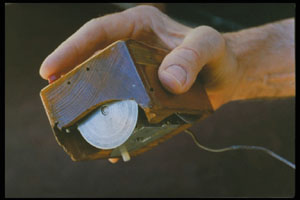
\includegraphics[width=0.3\linewidth]{figures/mouse.jpg}
	\caption{The first mouse}
\end{figure}

New and revolutionary ideas are required to create new peripherals that improve productivity, but are still intuitive and thus easy to learn to use. To get inspiration for improvement, one can look around and study already existing communication methods, for example the communication between humans. 

When two people are in a room and do not have an auditive or visual limitation, they will probably communicate by speech. But there is much more going on than only producing and interpreting words. The intonation, speed and other small variations in the voice add a lot more information to the words. Also the facial expression and body language give more space for expression. Some people like to `talk with their hands' while telling a story, something that adds more expression to the transmitted information.

\subsection*{Sign Language}

A deaf person cannot interpret spoken words, at least not by listening. He or she is highly depended on visual information. Sign languages have been emerged or invented to aid this visual communication. In these languages two elements play an important role: the face and the hands. These body parts give the most expressive power. The face because it is very good for expressing feelings and emotions, and the hands because they are very deformable. This makes the hands very interesting and useful, since there are countless combinations of finger poses and orientations. 

Speech synthesis \citep{Hunt1996}, speech recognition \citep{rabiner1993}, facial expression recognition \citep{Cohen2003} and sign language interpretation \citep{Cooper2007} are all subject of extensive research. Breakthroughs in these areas are important for revolutionary new interfaces which can tremendously improve the speed of interaction and usability for a user. 



This thesis aims at looking into the details of using computer vision to interpret sign language and especially to use sign language to actually control the computer - to use your hands for non-intrusive interaction. To show the advantages of having such a system it would be interesting to find an application for it and demonstrate that this can be actually useful. The application found was sound generation and manipulation, or in other words; making music. 

Translating sign language into music is a very interesting concept, not only because it sounds poetic but it can really demonstrate the power of such a system. Making live music is a complex process where real-time interaction between a artist and his tools is important. Also, for an audience it is much more compelling to look at a artist who is physically more active than only clicking a mouse.

\subsection*{Hand Poses}
Sign language does not really have distinct signs for musical concepts. Usually, when music is translated into sign language only the vocals are translated. Facial expression and references to emotions are used to indicate the `mood' of the music and the speed and expressiveness of the gestures indicate the intensity of the music, but these kind of gesture are not really usable for HCI because they are too subjective. A more formal method is required. Also, previous studies have shown that the segmentation of the consecutive gestures is a difficult task \citep{Buehler2009,RichardBowden2004}.

It is more feasible to have a limited set of hand poses that corresponds to a set of commands and parameters.  Any set of hand poses would do for this system, as long as the individual poses do not look too similar. Since the idea is to translate the interpreted hand poses into sound, it would be interesting to use a set of poses that has an already existing relationship to sound.

In Medieval music, the Guidonian hand was a mnemonic device used to assist singers in learning to sight sing; singing according to visual perceived information like sheet music or hand gestures, typically not seen before. The idea of the Guidonian hand is that each portion of one hand represents a specific note within the hexachord system, which spans nearly three octaves. The other hand is used to point to the correct hand portion. \autoref{fig:guidonian} shows a hands with the tonal positions.

\begin{figure}[tb]
	\centering{}
	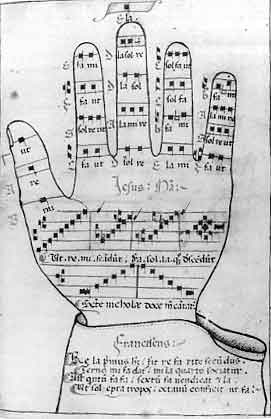
\includegraphics[width=0.3\linewidth]{figures/guidonian_hand.jpg}
	\caption{Guidonian Hand}
	\label{fig:guidonian}
\end{figure}

Despite the fact that this system has a large set of symbols - 22 to be exact - this system is not usable since the individual poses are very much alike. Discriminating between the different positions on the hand will be problematic.

A more recent method using hand poses in relation to music are the Curwen solfege hand signs \citep{choksy1999}. This method was introduced in the 19th century by John Curwen, who also is the founder of the famous tonic sol-fa. The tonic sol-fa is better known as \emph{'do re mi fa sol la ti'}.

\begin{figure}[tb]
	\centering{}
	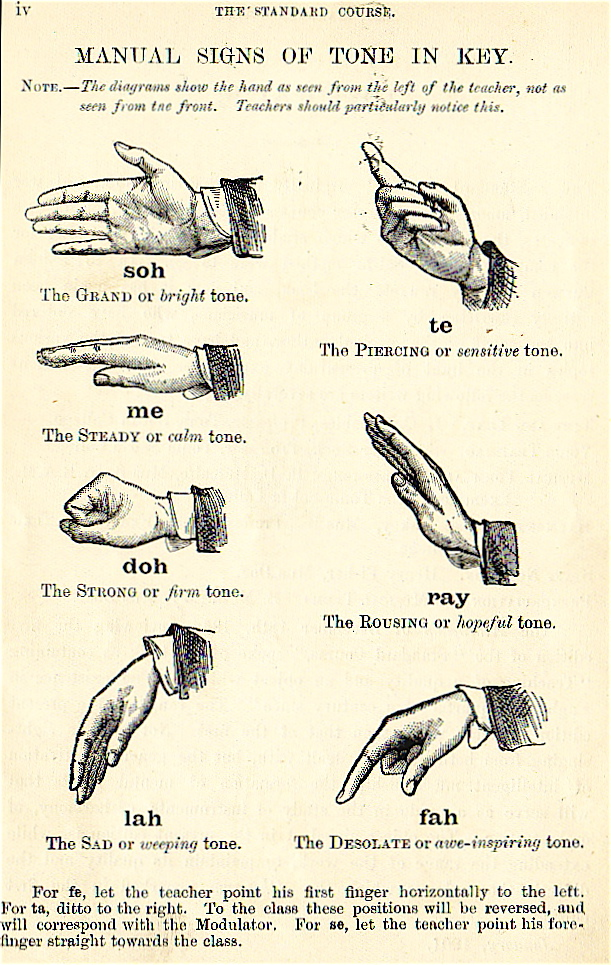
\includegraphics[width=0.4\linewidth]{figures/curwen.jpg}
	\caption{Depiction of Curwen's Solfege hand signs from 1904}
	\label{fig:curwen}
\end{figure}

\autoref{fig:curwen} is a scan from a teaching book from 1904 where the 6 tonal hand poses are shown. These 6 poses correspond to the 6 notes in the musical major scale. These hand poses are much more suitable for our system, since the individual hand symbols are distinct. Also the hand poses can be easily performed by both hands individually next to the body or in front of the body. \autoref{fig:curwennotes} shows the same hand poses with the corresponding musical tones. It is less common known that there are also names for the chromatic increase and decrease, flat ($\flat$) or sharp ($\sharp$) tones. These names are \emph{'di, ri, fi si li'}. Also these tonal names have their own corresponding Curwen hand poses.

\begin{figure}[tb]
	\center{}
	\subfloat{
		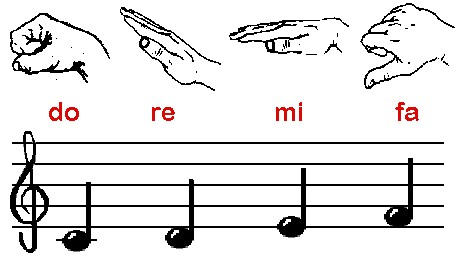
\includegraphics[width=0.45\linewidth]{figures/doremifa.jpg}
	}
	\hspace{0.03\linewidth}
	\subfloat{
		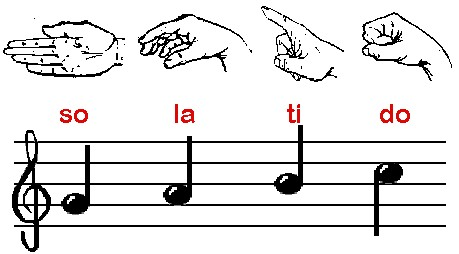
\includegraphics[width=0.45\linewidth]{figures/solatido.jpg}
	}
	\caption{The curwen hand symbols and the corresponding musical notes}
	\label{fig:curwennotes}
\end{figure}


\section{The Goal}
\label{sec:goal}
The goal of this thesis is to describe the design and evaluation of a system for hand pose recognition. The system needs to be fast and user friendly; it should be able to run on current consumer hardware. Overall the system should satisfy the following requirements:

\begin{itemize}
	\item Localize and interpret the hand poses of a person in a video stream
	\item Do this with real time performance; a minimum of 10 frames per second (FPS). 10 FPS is enough for the human perception to perceive consecutive images as a movie. 
	\item Processor power requirements should be moderate; it needs to work on a normal consumer desktop or laptop
	\item Use a normal inexpensive RGB camera or webcam, without infrared
	\item Non-intrusive, no gloves or skin mounted electromechanical sensors
	\item No calibration or initialization is required at startup or during the usage
	\item Minimal to no configuration parameters are desired.
\end{itemize}
	
To realize these requirements some restrictions on the system's setting are required:

\begin{itemize}
	\item There should be only one person at a time in the image
	\item The person is wearing clothing with long sleeves, no arm skin is visible
	\item The lightning conditions should be `good enough', enough light should illuminate the user
	\item There should be no skin like colors in the image like pictures and posters with faces.
\end{itemize}

The system can be used as a controller for a computer, with a focus on subtle detail for continuous variables, which give the sense of more direct control which is important for real time interaction. Akin to how a graphical designer prefers a graphics tablet over a mouse for drawing, the design of the system aims to accomplish a similar sensation. The output of the system can be easily configured by a user to map to his or her preferred set of commands. For example, one hand can control the pitch of a sound, while the other controls an accompanying beat while the position of this hand controls a sound manipulating variable.

It is important to say that the scope of this thesis is limited to extracting the hand poses from video, and will not cover the study of the mapping of hand poses into sound although a prototype system is discussed in chapter \autoref{ch:sonicgesture}.


\section{Related Work}
At the moment of writing this thesis Microsoft is finishing the development of a new commercial product called `Kinect'. Kinect is claimed to provide full-body 3D motion capture. To accomplish this, Kinect uses a range camera, which interprets 3D scene information from a continuously-projected infrared pattern. For this setting an infrared projector and a range camera is required. It is interesting to see that again (this is also the case for the Wii) a new revolutionary input device is created for a gaming console. 

\begin{figure}[tb]
	\center{}
	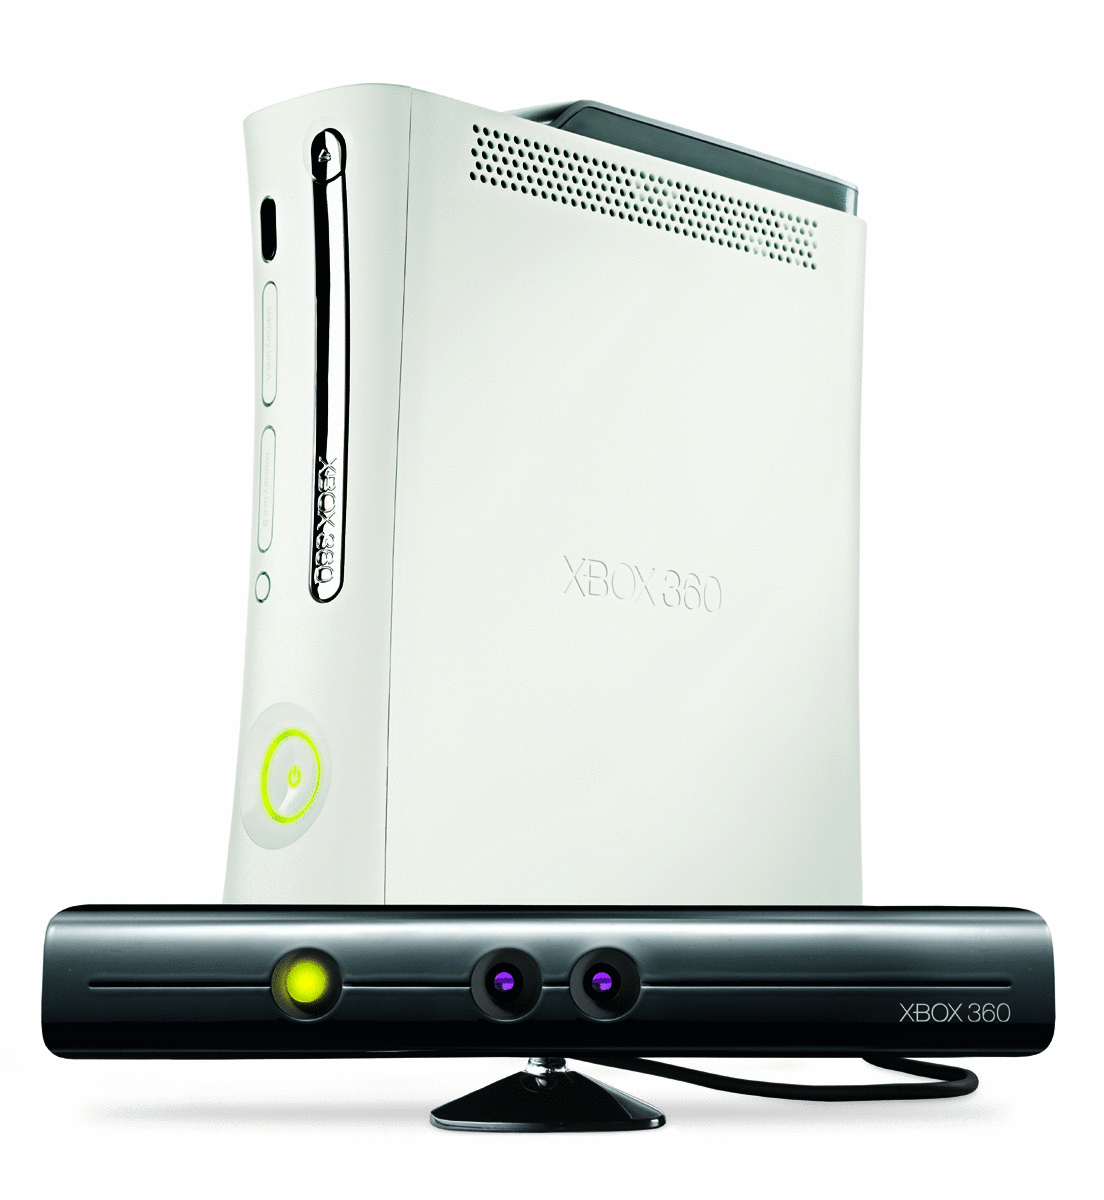
\includegraphics[width=0.3\linewidth]{figures/wave.jpg}
	\caption{Microsoft Kinect}
	\label{fig:kinect}
\end{figure}

\citep{Yi2009} proposed a method for computer aided 3d architecture design using hand gestures, see \autoref{fig:yi2009} for the a model constructed with this software.

\begin{figure}[tb]
	\center{}
	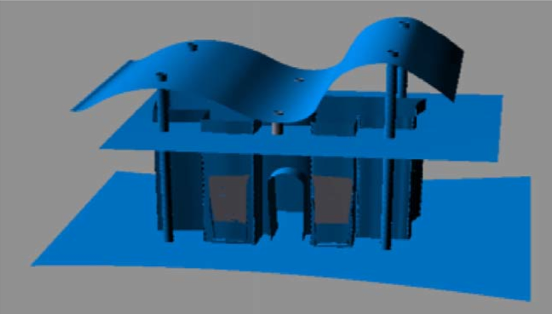
\includegraphics[width=0.6\linewidth]{figures/yi2009.png}
	\caption{3D model of train station made with aid of hand gestures}
	\label{fig:yi2009}
\end{figure}

A lot of work has been done in the field of hand pose recognition. \citep{Erol2007,Mitra2007} give a good overview of what has been done and what techniques have been used.

A similar approach as described in this paper is \citep{Wang2007}, but SIFT features are used and only 3 hand poses are detected. From the same author is \citep{Wang2009}, where a colored glove \autoref{fig:wang2009} is used to perform full 3d hand pose estimation which seem to yield promising results. The disadvantage of this method is the intrusive requirement of wearing a specific color glove, see \autoref{fig:wang2009}.

\begin{figure}[tb]
	\center{}
	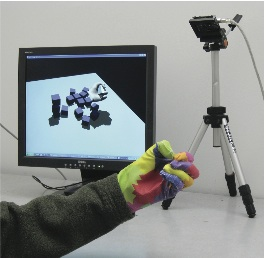
\includegraphics[width=0.4\linewidth]{figures/wang2009.jpg}
	\caption{3D hand pose estimation using a colored glove}
	\label{fig:wang2009}
\end{figure}

\citep{Segen1999} used shadows of hand poses for pose estimation. \citep{Mo2006} proposes a method for pose estimation from low-resolution depth images from a laser camera. A 3d model fitting approach is described in \citep{Athitsos2003,laGorce2010}. \citep{Stenger2006} uses template matching for pose estimation. \citep{Xiong2006} describes a method for 3d hand path tracking in a meeting setting with multiple camera's. \citep{Nickel2007} proposes a method for detection pointing gestures with a single camera.

\citep{Hassanpour2008} describes an adaptive skin color segmentation method using Guassian Mixture Models. \citep{Phung2002} talks about skin modeling in the YCbCr color space and the application to human face detection. \citep{Sigal2004,Soriano2000,Stoerring1999} discuss the handling of changing illumination. \citep{Kakumanu2007} is a survey paper about skin color modeling and detection.

An alternative approach to hand localization than described in this thesis is to capture the complete body pose. This could be a more robust method, but is at the moment computationally expensive. \citep{ferrari2008} introduces a method to extract a body pose from monoscopic video. \citep{VandenBergh2009} proposes a method for 3D pose recognition using multiple camera's. \citep{Poppe2007} discusses how 3D model fitting can be used for pose estimation. \citep{Moeslund2006} gives an overview of all relevant body pose estimation research until 2006.

\citep{Buehler2009} discusses a method to learn sign language with news broadcasts that are subtitled and translated into sign language. The complexity of segmentation in sign language is discussed in \citep{RichardBowden2004}. An other approach for segmentation is discussed in \citep{Cooper2007}. \citep{starner1998,Vogler1999} use Hidden Markov Models to model sign language.





